\section{Recording Environments} \label{sec:meth_RecordingEnvironments}

This section will explain the first step in the data acquisition pipeline detailed above \ref{sec:meth_DataAcquisitionPipeline}, namely the two recording environments. Their function is to interface with Tobii ET5 to extract raw eye movement data and organize it in a structured dataset. Additionally, the dataset is pre-labeled with approximate eye movement event labels to simplify the manual post-labeling process.

Both recording environments are implemented in \texttt{.NET Core 3.1} using \texttt{C\# 8.0}. Interfacing with Tobii ET5 is done with an API-wrapper implemented in \texttt{.NET Framework 4.8} using \texttt{C\# 7.3}.

% In this section, I will describe the various methods used for data labelling, each with its purposes and advantages. 

% \textit{The methods used will be compared and finally used for training a classification model.}

\subsection{Static}

A scaled-down version of the static recording environment is shown in figure \ref{fig:meth_StaticLabellingEnv}. It is intended to run full screen on the recording monitor. It consists of a single large image, two on-screen buttons, an instructional text, and a tracking status indicator. One button enables and disables the eye-tracking data stream, after which a heat map and a time-series data file are generated. A second button determines how outgoing data samples are pre-labeled. Possible labels are fixation, saccade, and blink. The button is interactable to indicate when the user is fixating somewhere on the image or blinking. On-screen stimulus is in the form of a highly abstract and visually stimulating image. It is chosen so no area of particular interest draws the user's attention since that might introduce unwanted bias in the data.

\begin{figure}[h]
    \centering
    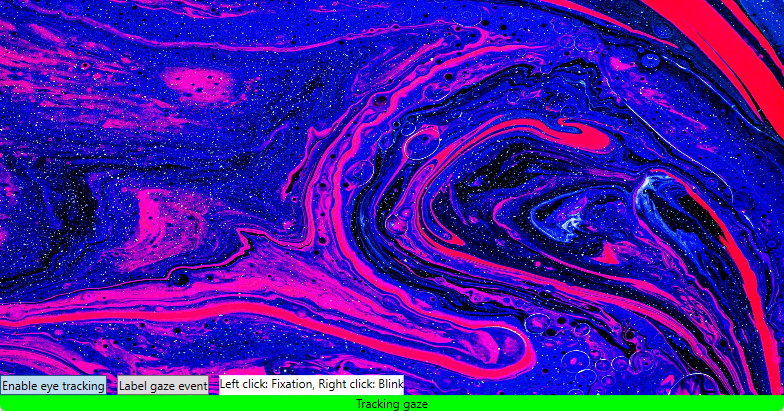
\includegraphics[width=\textwidth]{Images/Labelling/StaticEnvironment2.png}
    \caption{Static labelling environment, used to label data for the binary classification problem.}
    \label{fig:meth_StaticLabellingEnv}
\end{figure}


% For binary classification, we limit the model to only classify whether a sample represents a saccade or not. As such, the labelling environment required can be limited to one where only saccades are labelled, whereas  all other samples can be directly labelled as fixations. This allows for a very simple system for data labelling, where the user is asked to manually indicate when he is adjusting his gaze point.

% Unfortunately, this way of labelling data introduces bias by human error. An ideal ground truth should be impeccable in its classifications, as the machine learning classification model can never be better than the dataset from which it trains its parameters. For this reason, we introduce a manual post-labelling step, where an operator scans through the labelled samples and correct erroneous labels by observing the onset and offset of differences in recorded on-screen xy-coordinates.

\subsection{Dynamic}

The dynamic recording environment improves upon the above by replacing static stimulus with a graphical element able to animate the movement of a white dot on a black screen. Movements are random within some constraints and include instantaneous warping and slow displacements. Displacements are along straight lines or second-degree parabolas and between two and five seconds in duration. The dot rests for at least two seconds between displacements. For every rest and movement of the stimulus, outgoing data samples are pre-labeled with either fixation, saccade, or smooth pursuit. An example snapshot of the environment, where the moving dot leaves a path along with its movement, is shown in figure \ref{fig:meth_DynamicLabellingEnv}. This figure also depicts the heat map that came from that particular recording. A heat map and a time-series data file are generated upon exiting the application.

\begin{figure}[h]
    \centering
    \begin{minipage}{0.5\textwidth}
        \centering
        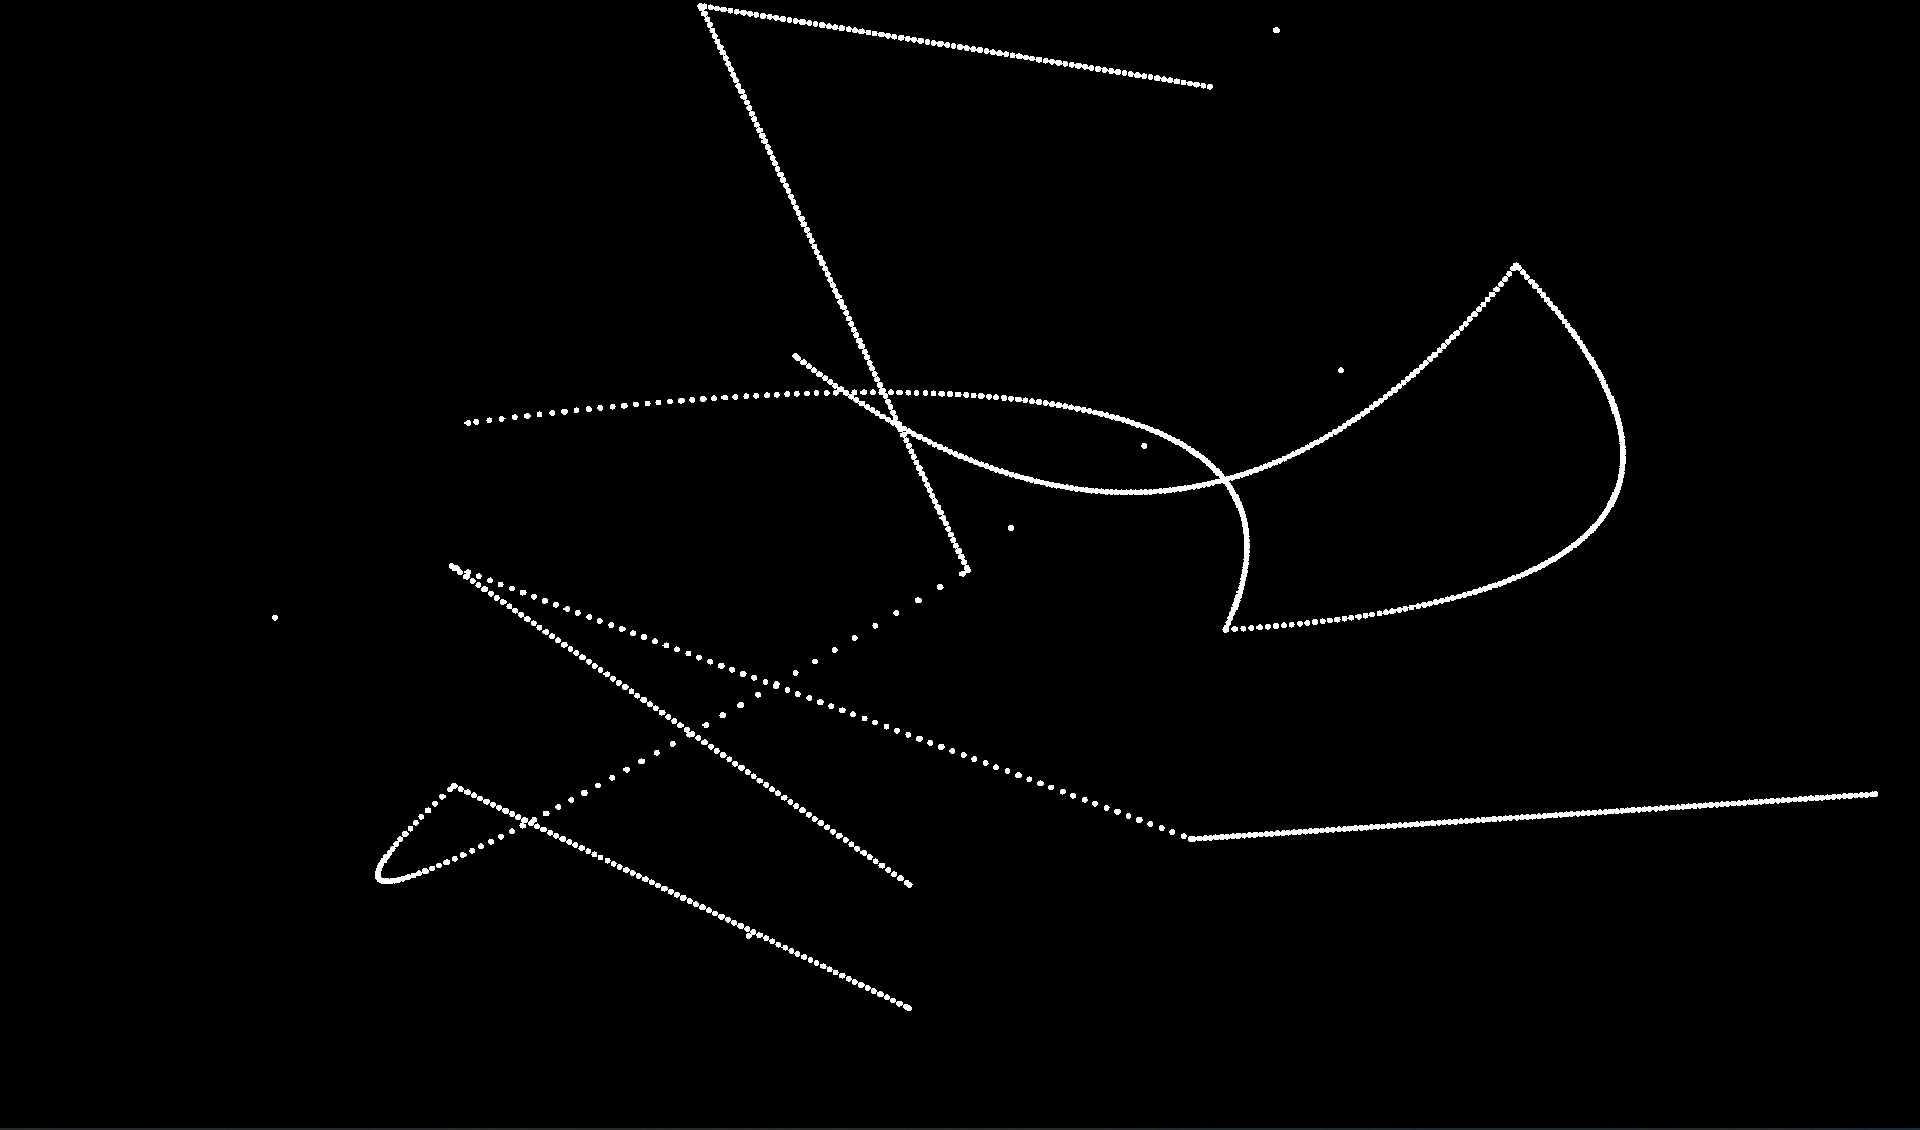
\includegraphics[width=\textwidth]{Images/Labelling/DynamicEnvScreen.png} % first figure itself
        %\caption{first figure}
    \end{minipage}\hfill
    \begin{minipage}{0.5\textwidth}
        \centering
        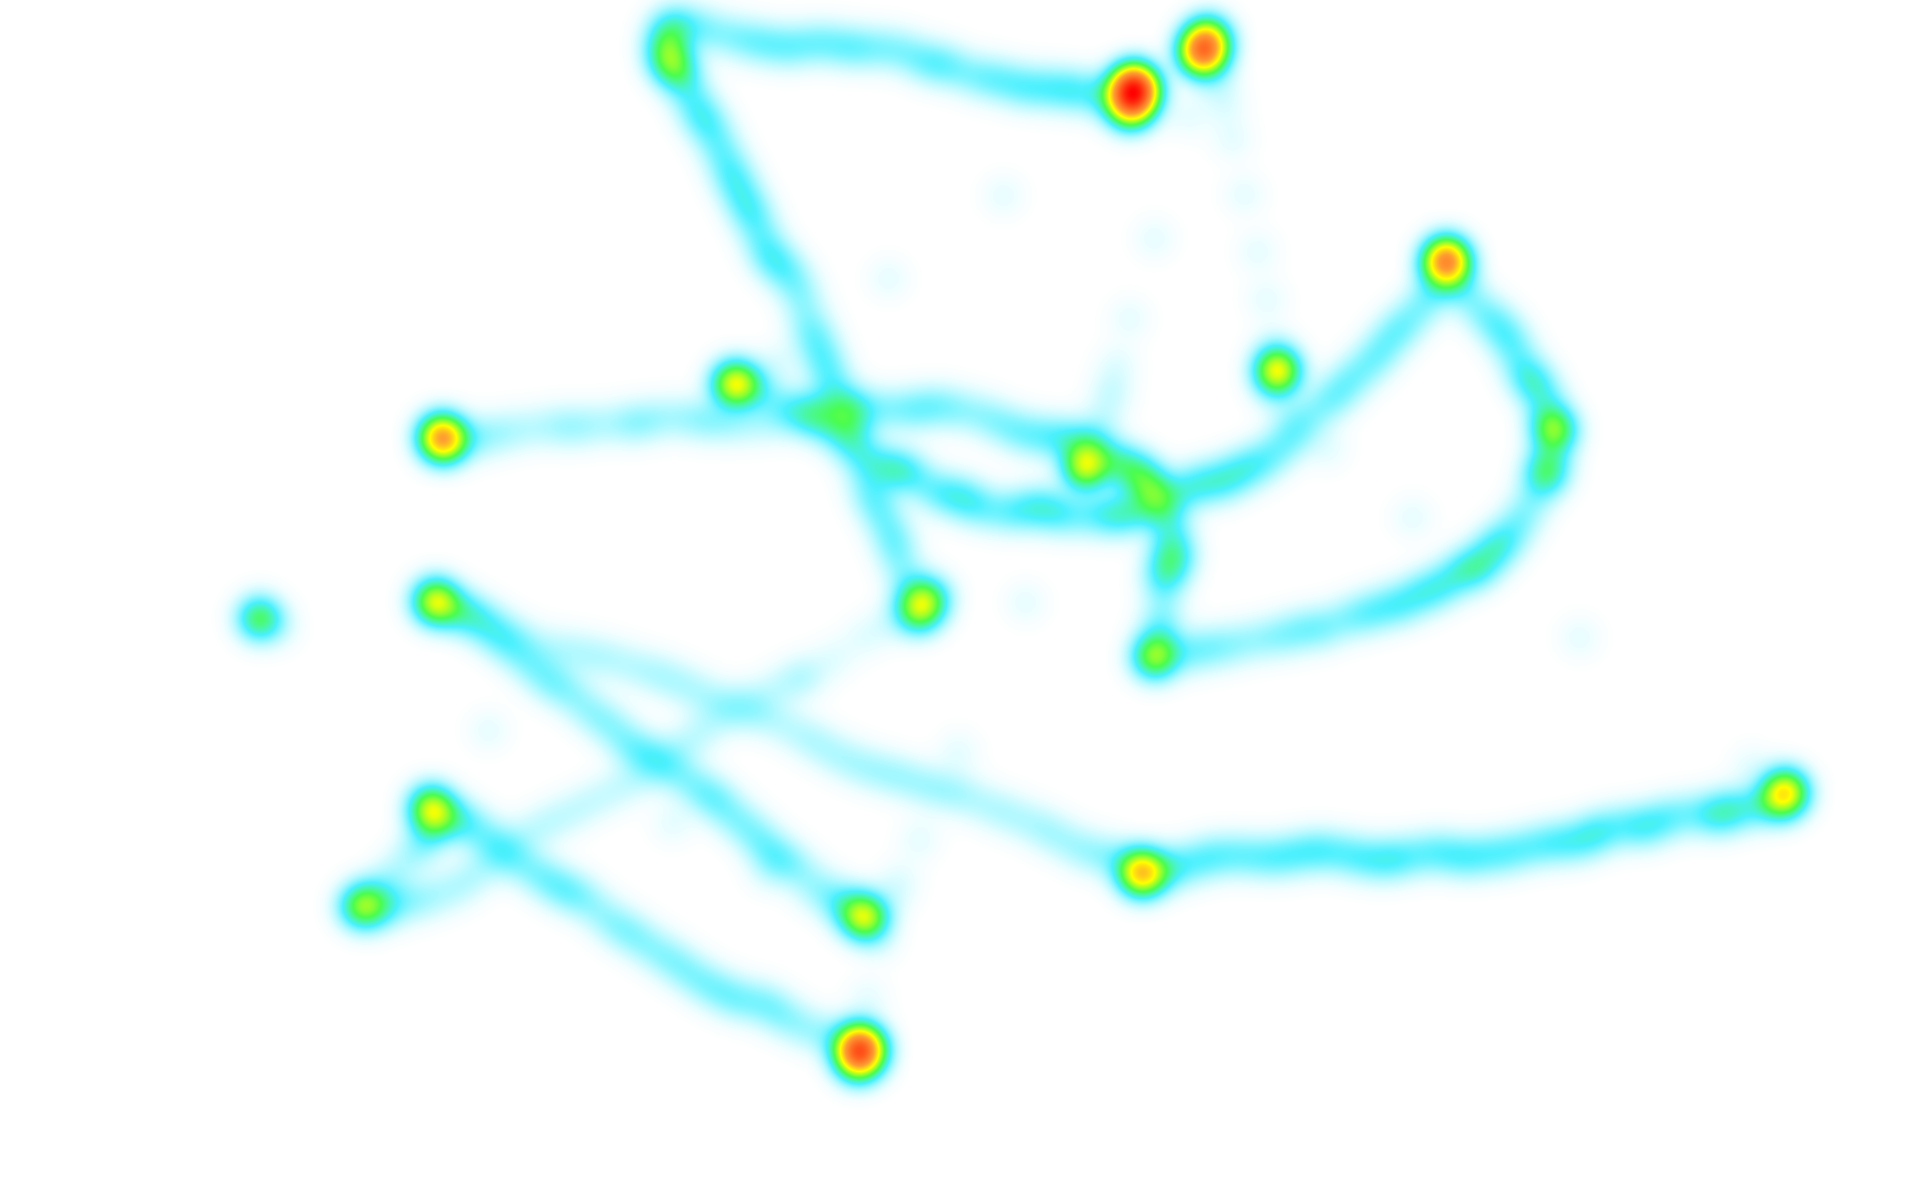
\includegraphics[width=\textwidth]{Images/Labelling/DynamicEnvHm.png}% second figure itself
        %\caption{second figure}
    \end{minipage}
    \caption{Dynamic Labelling environment. Left image represents the paths drawn by warping and moving dot during data recording. Right image is the heat map resulting from the same recording. Note that this example is artifially created to draw lines along displacement paths. During normal operation, there is only one dot on-screen at any time.}
    \label{fig:meth_DynamicLabellingEnv}
\end{figure}
